\begin{frame}[c]
\begin{center}
\Huge Classifier training
\end{center}
\end{frame}

\begin{frame}{Setup of the classifier}
\begin{block}{Hyper-parameter scan results}
\begin{itemize}
\item Input: \num{14} variables motivated by a BDT variable scan.
\item Hidden layers: \num{6} \ELU layers $\times$ \num{128} nodes each
\item Output layer: \num{1} \SIGMOID node
\item Optimisation: SGD, Learning rate $=0.06$, momentum $=0.3$, no nesterov, no decay
\item Duration: 600 epochs
\end{itemize}
\end{block}
\begin{block}{Variables}
\begin{itemize}
    \item Motivated by a BDT significance scan
    \item Tested against simple kinematic variables
\end{itemize}
\end{block}
\end{frame}

\begin{frame}{Simple network results}
\vspace{-4mm}
\begin{figure}[htbp]
    \centering
    \begin{subfigure}[b]{0.4\textwidth}
        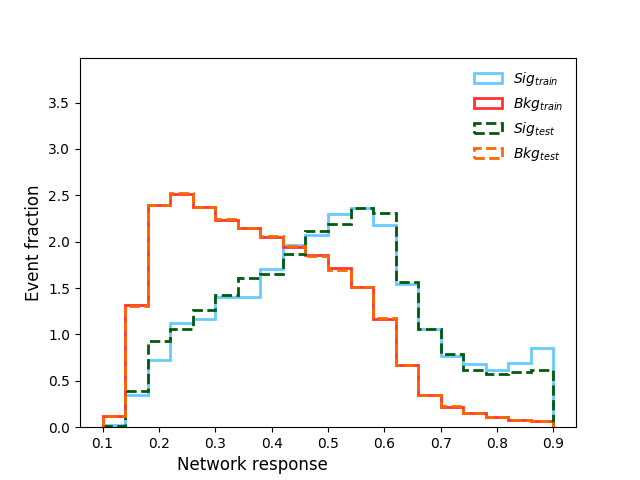
\includegraphics[width=\textwidth]{standard_separation}
        \caption{Separation}
        \label{fig:simple:final:sepa}
    \end{subfigure}
\quad
    \begin{subfigure}[b]{0.4\textwidth}
        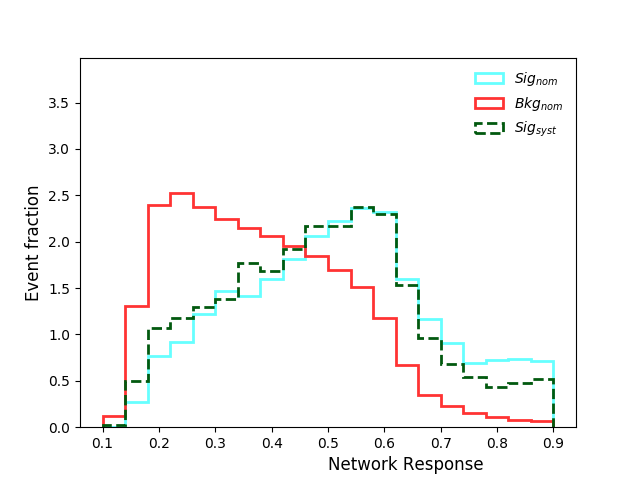
\includegraphics[width=\textwidth]{standard_syst}
        \caption{Systematics}
        \label{fig:simple:final:syst}
    \end{subfigure}

    \begin{subfigure}[b]{0.4\textwidth}
		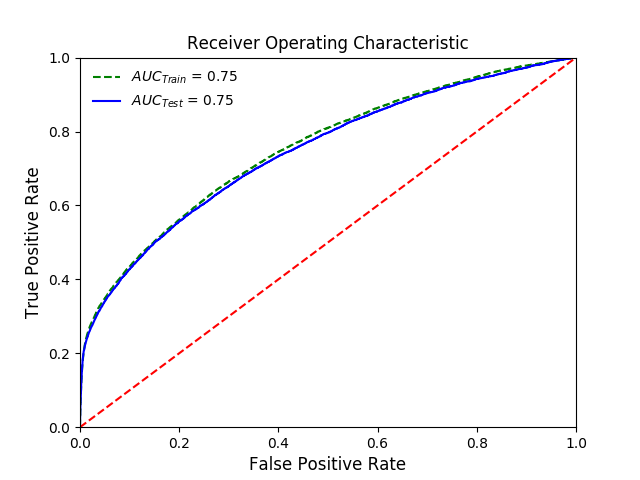
\includegraphics[width=\textwidth]{standard_ROC}
		\caption{ROC curve}
		\label{fig:simple:final:roc}
	\end{subfigure}
\quad
	\begin{subfigure}[b]{0.4\textwidth}
		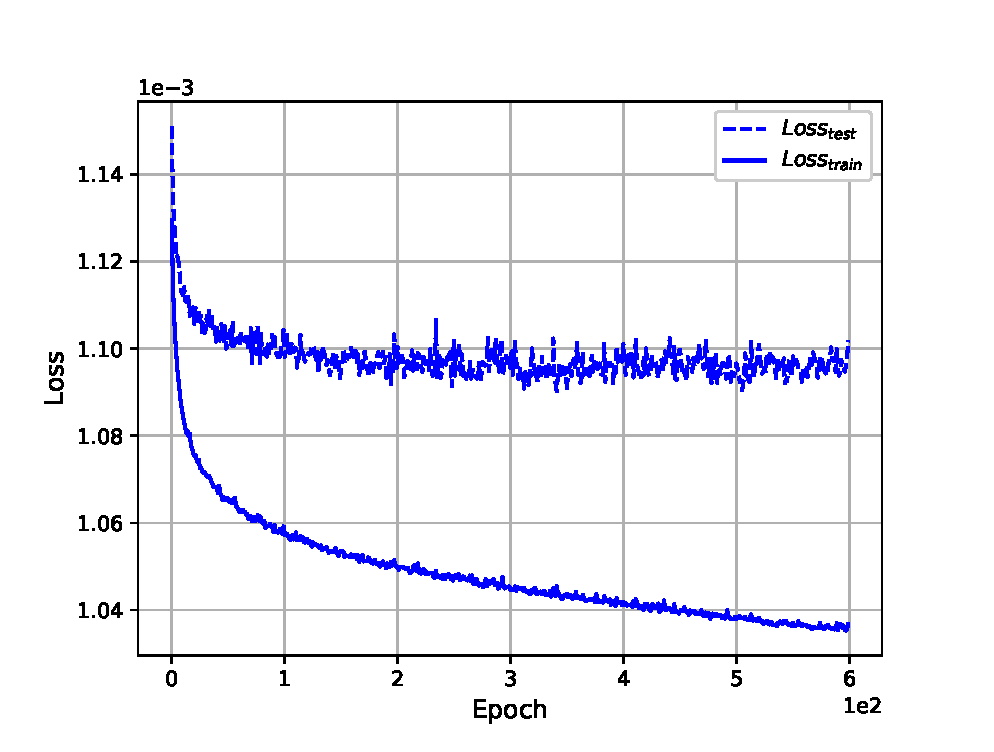
\includegraphics[width=\textwidth]{standard_losses}
		\caption{Losses}
		\label{fig:simple:final:loss}
	\end{subfigure}
\end{figure}
\end{frame}